\section{Beispiele}

\newpage
\begin{figure}[h]
	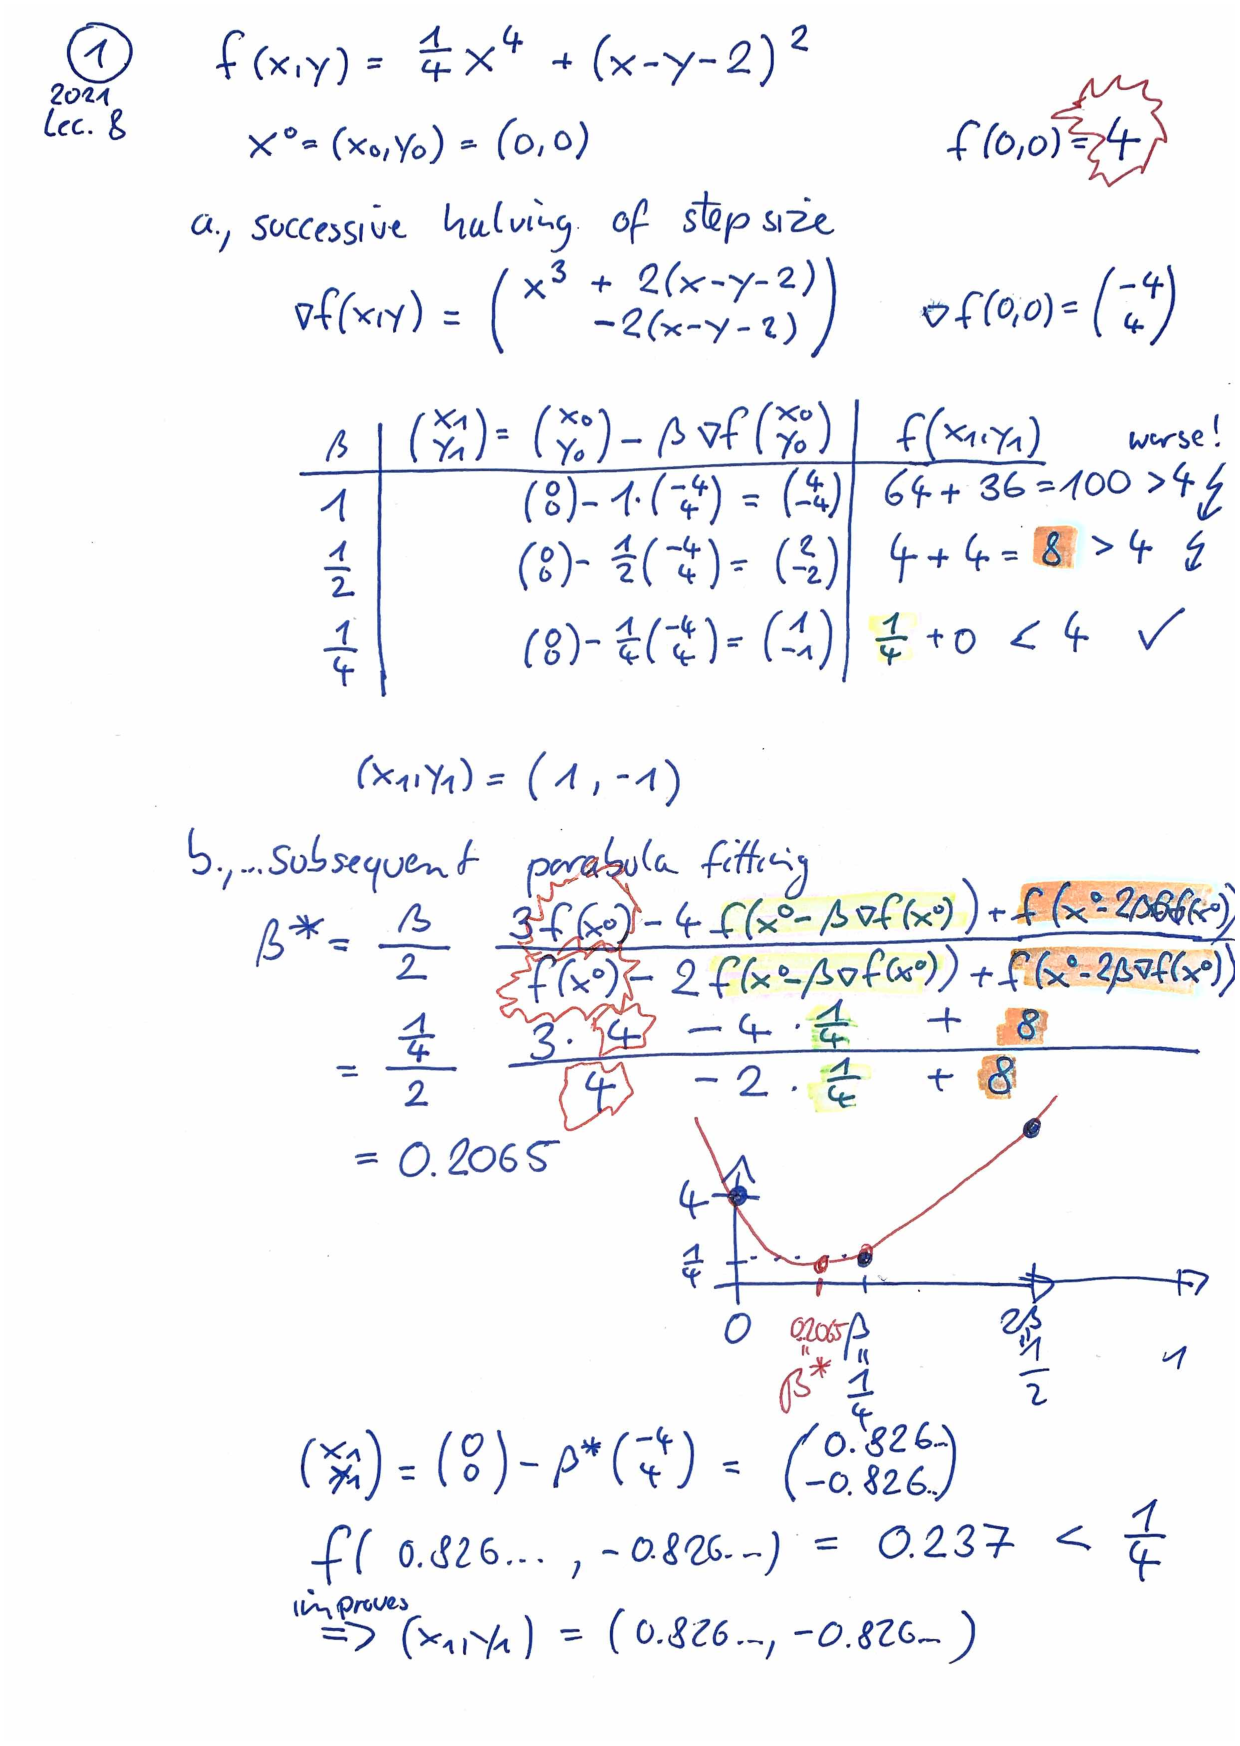
\includepdf[pages=1]{./Content/Examples/example-gradient-descent.pdf}
\end{figure}

\newpage
\begin{figure}[h]
	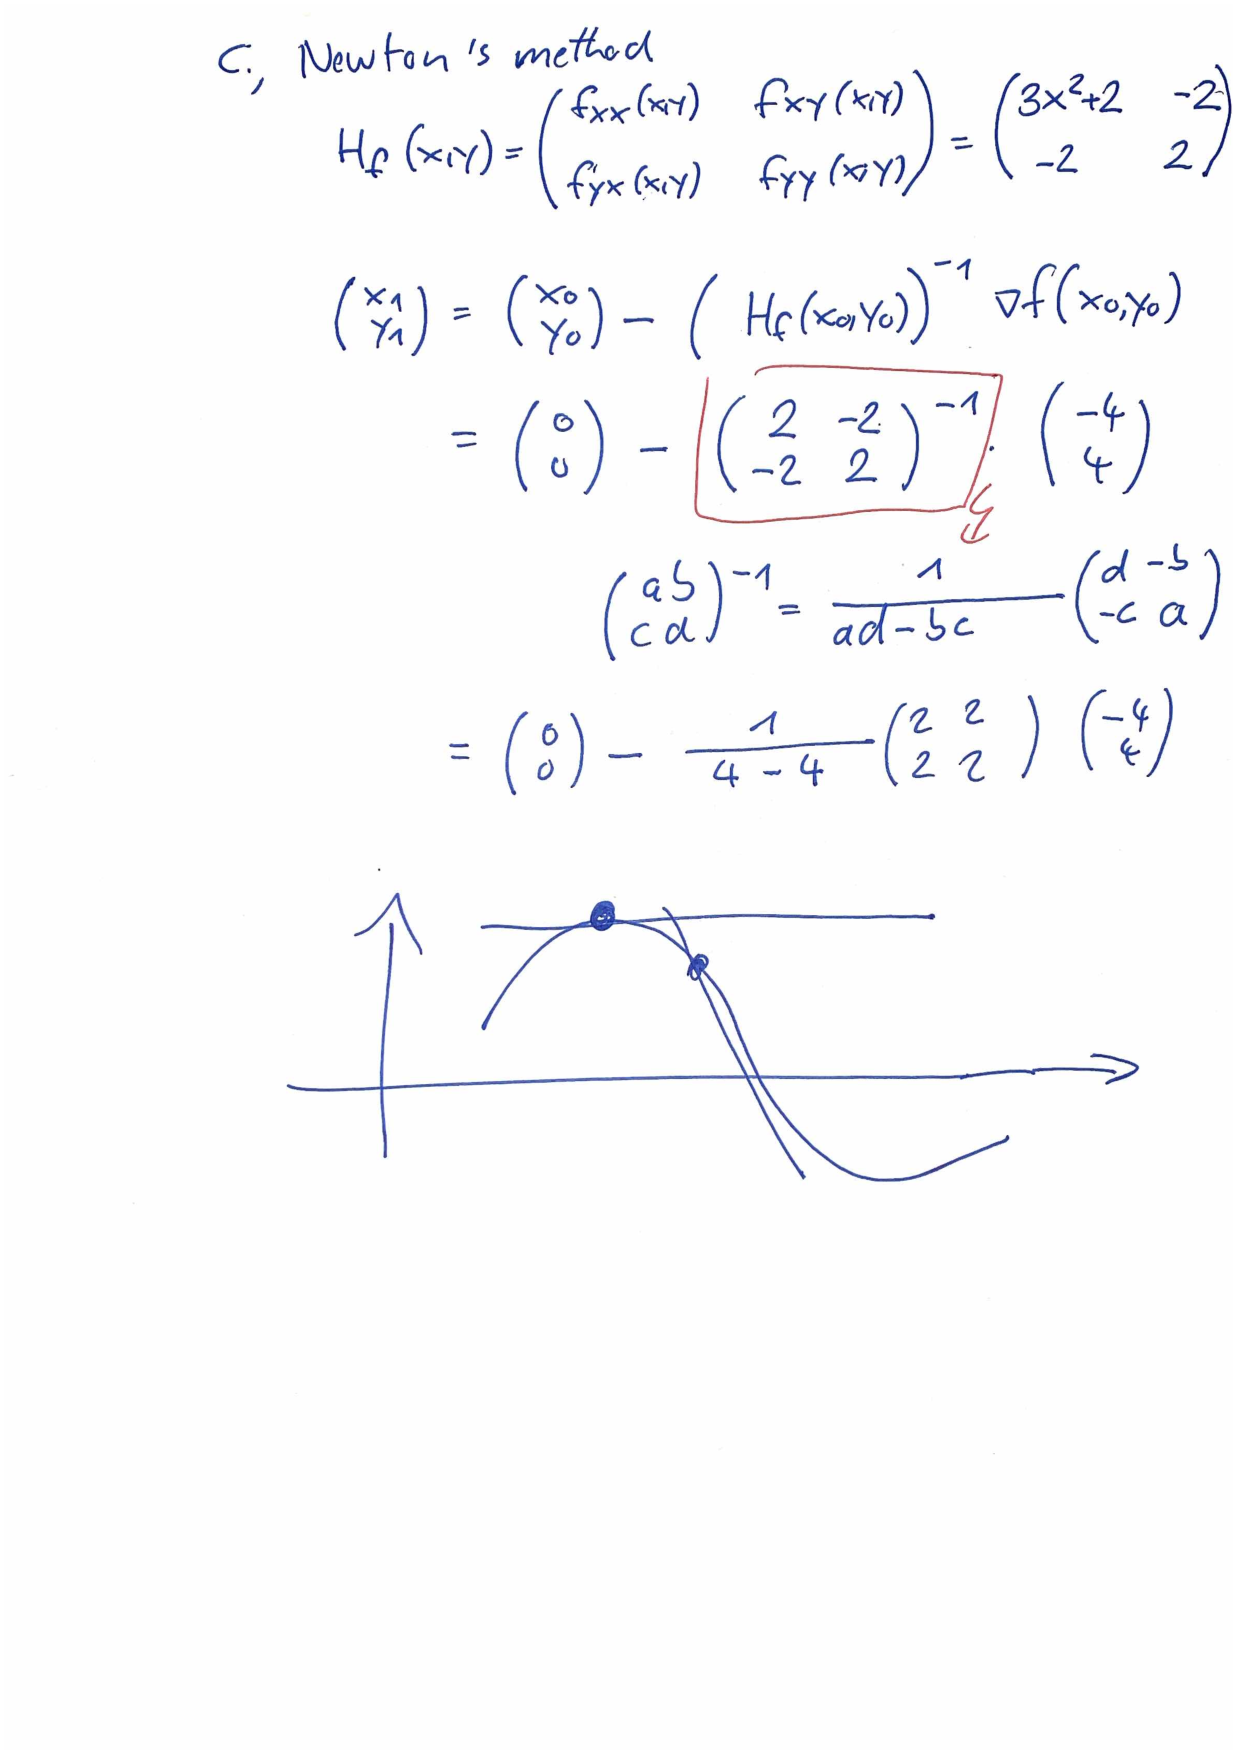
\includepdf[pages=1]{./Content/Examples/example-newton.pdf}
\end{figure}

\newpage
\begin{figure}[h]
	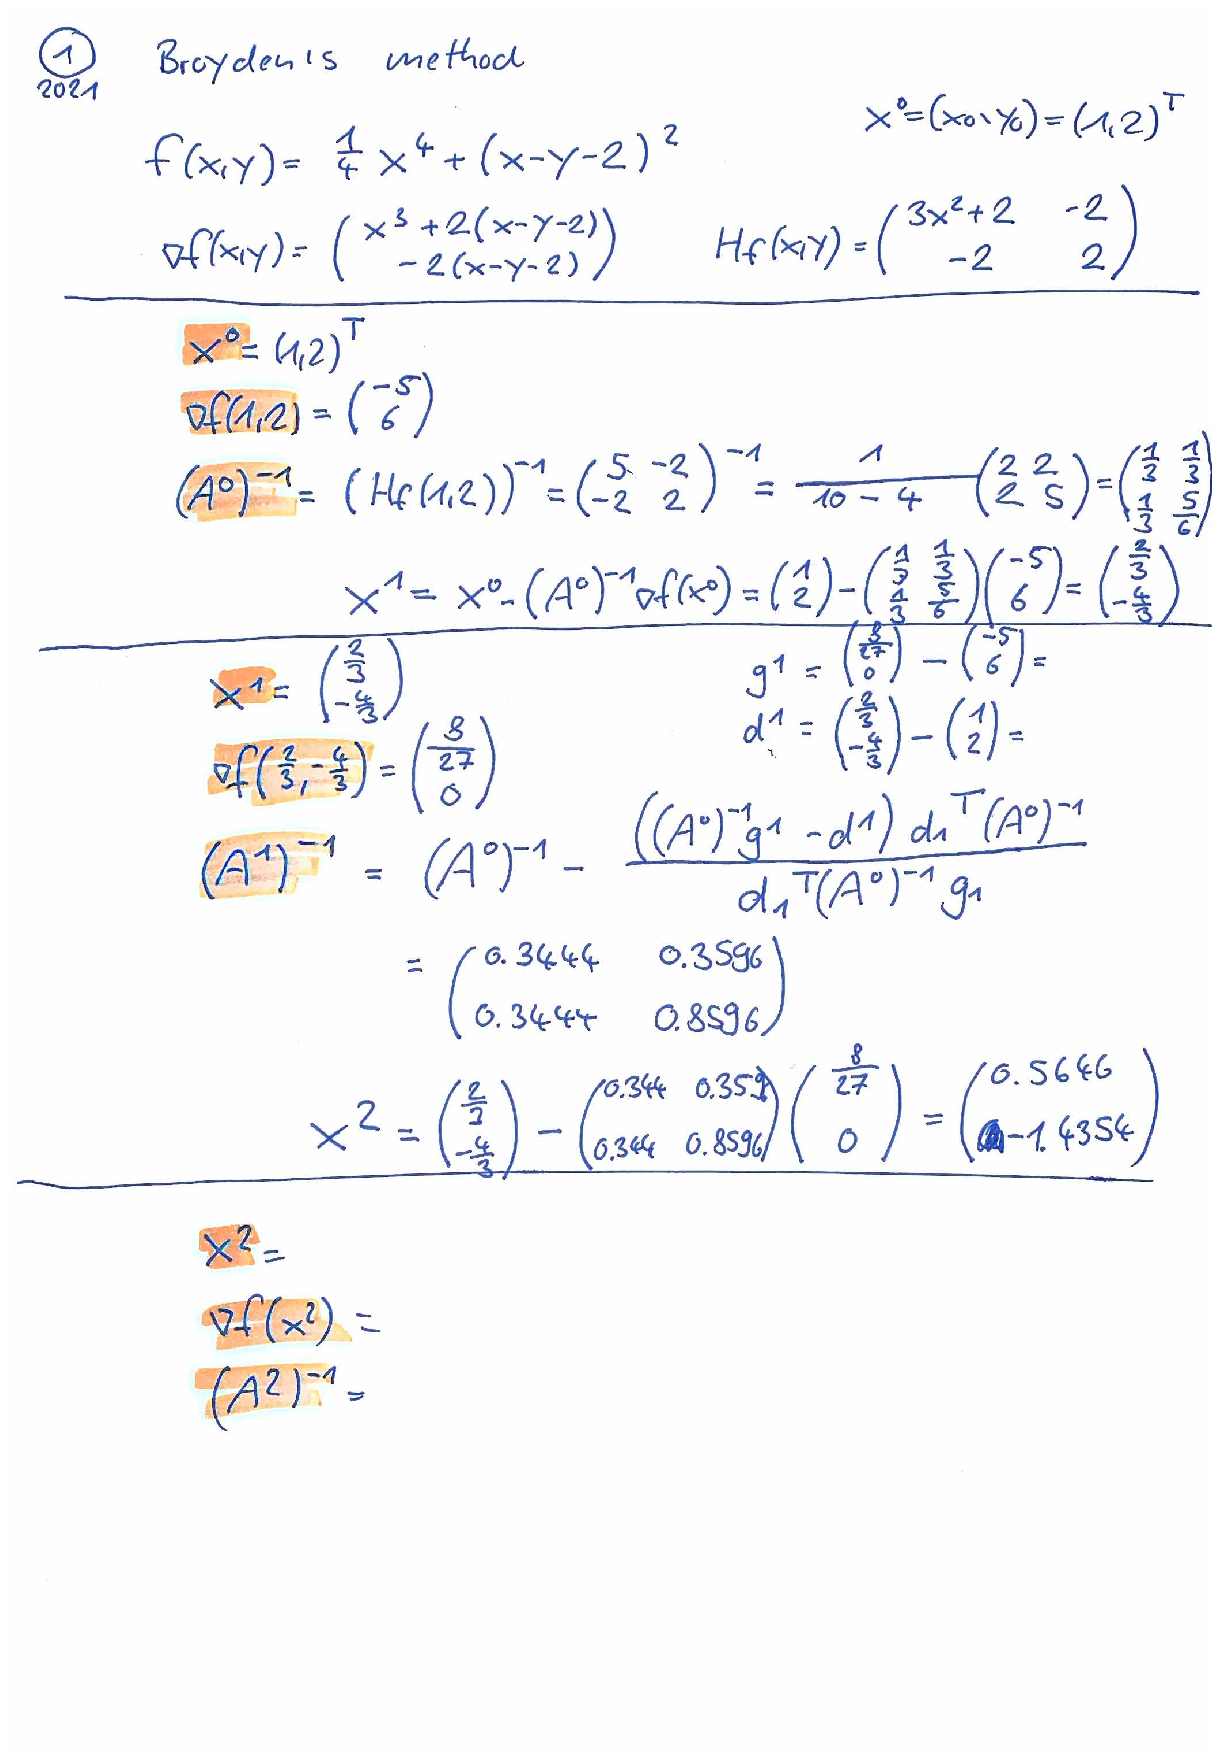
\includepdf[pages=1]{./Content/Examples/example_broyden.pdf}
\end{figure}

\newpage
\begin{figure}[h]
	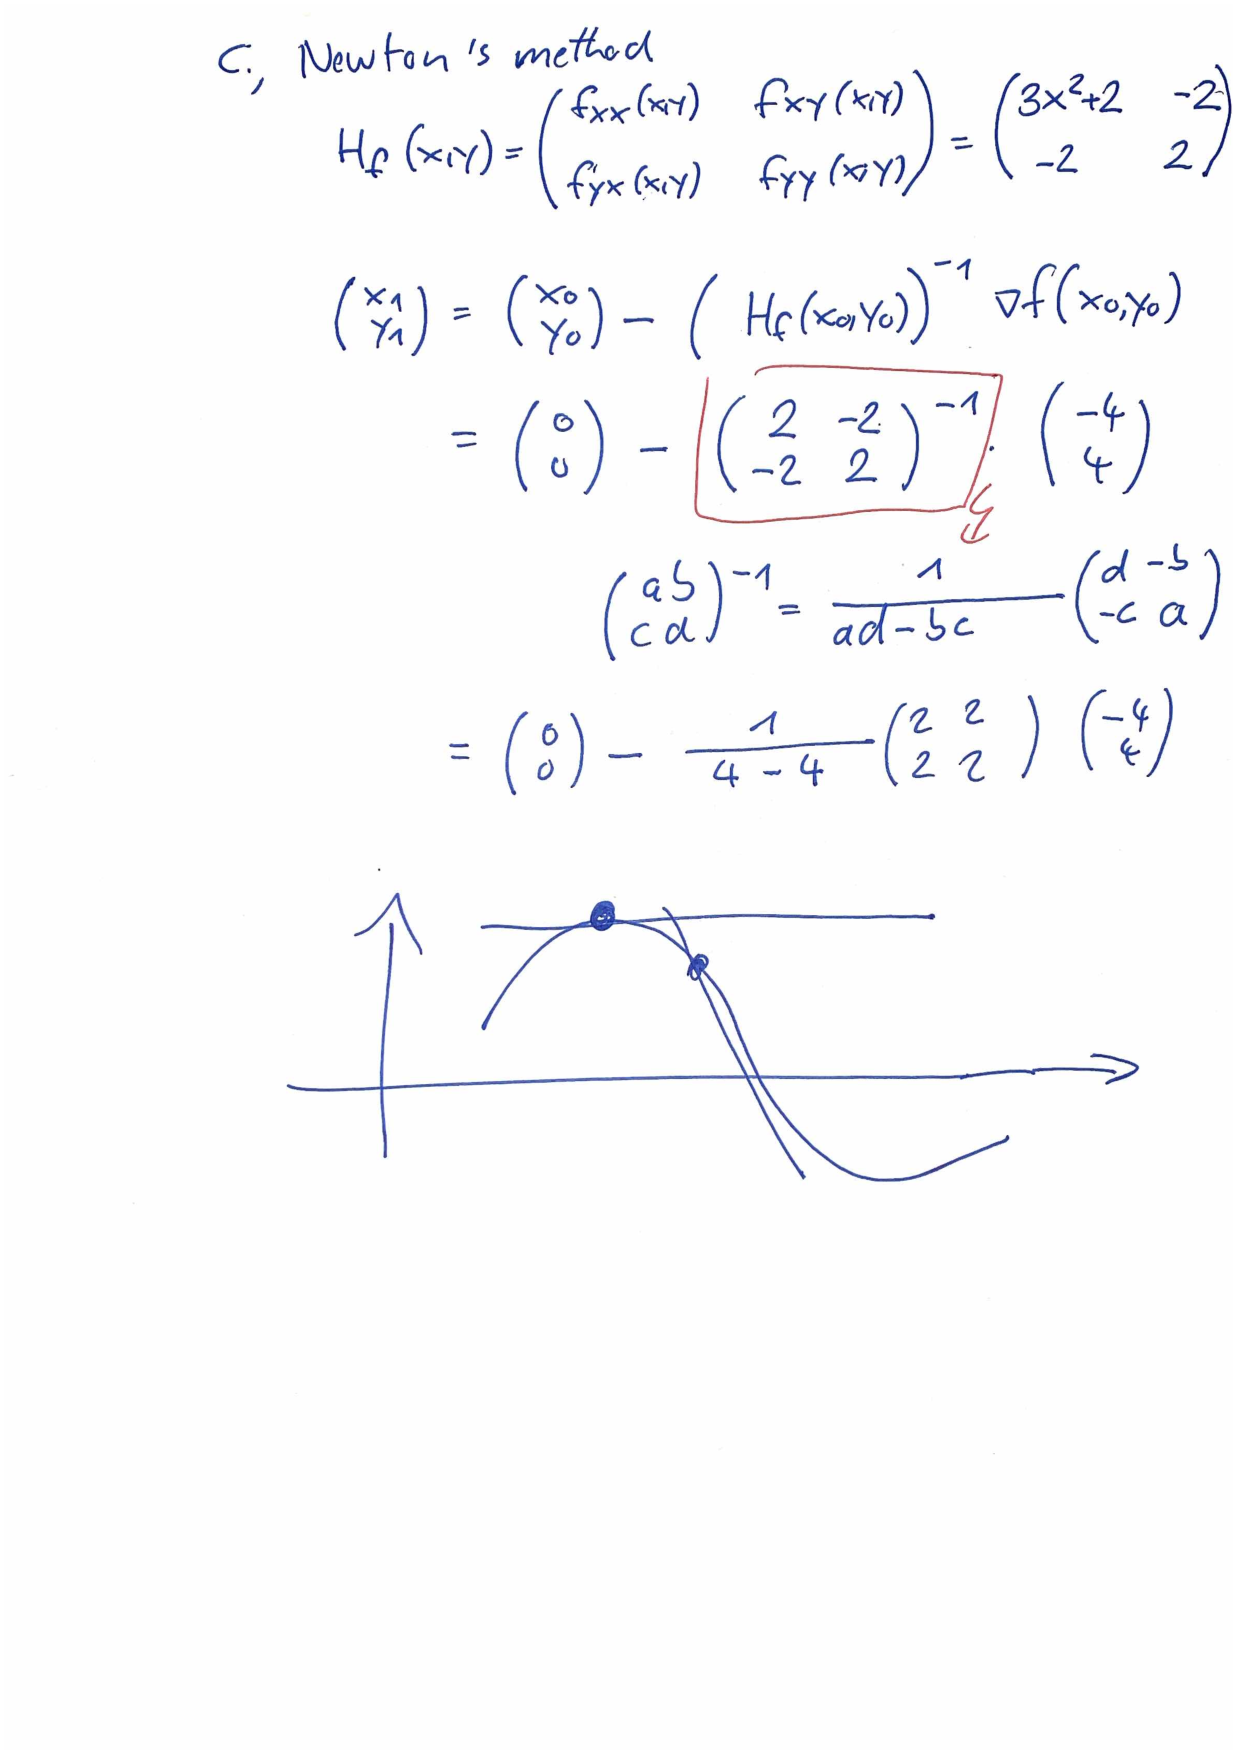
\includepdf[pages=1]{./Content/Examples/example-newton.pdf}
\end{figure}

\newpage
\begin{figure}[h]
	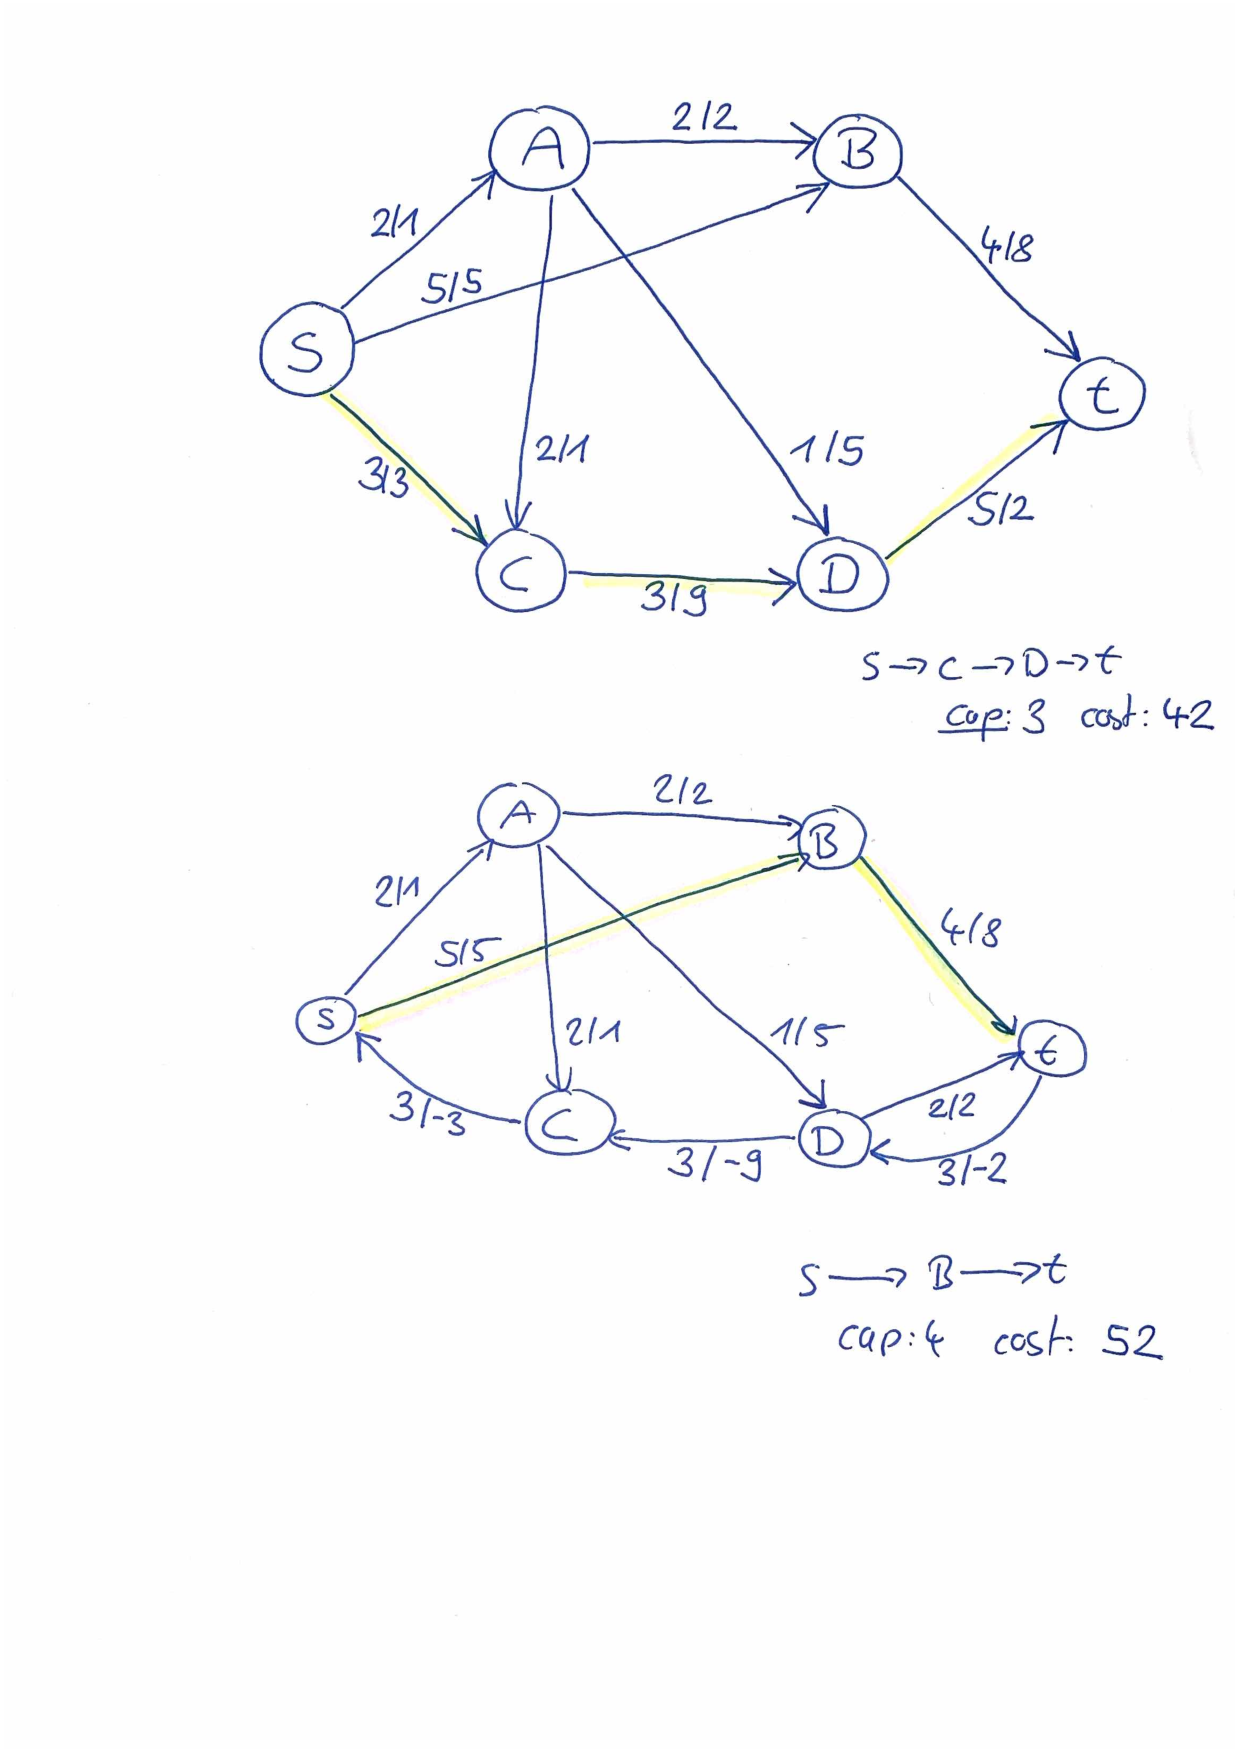
\includepdf[pages=1]{./Content/Examples/example_maxflow1.pdf}
\end{figure}

\newpage
\begin{figure}[h]
	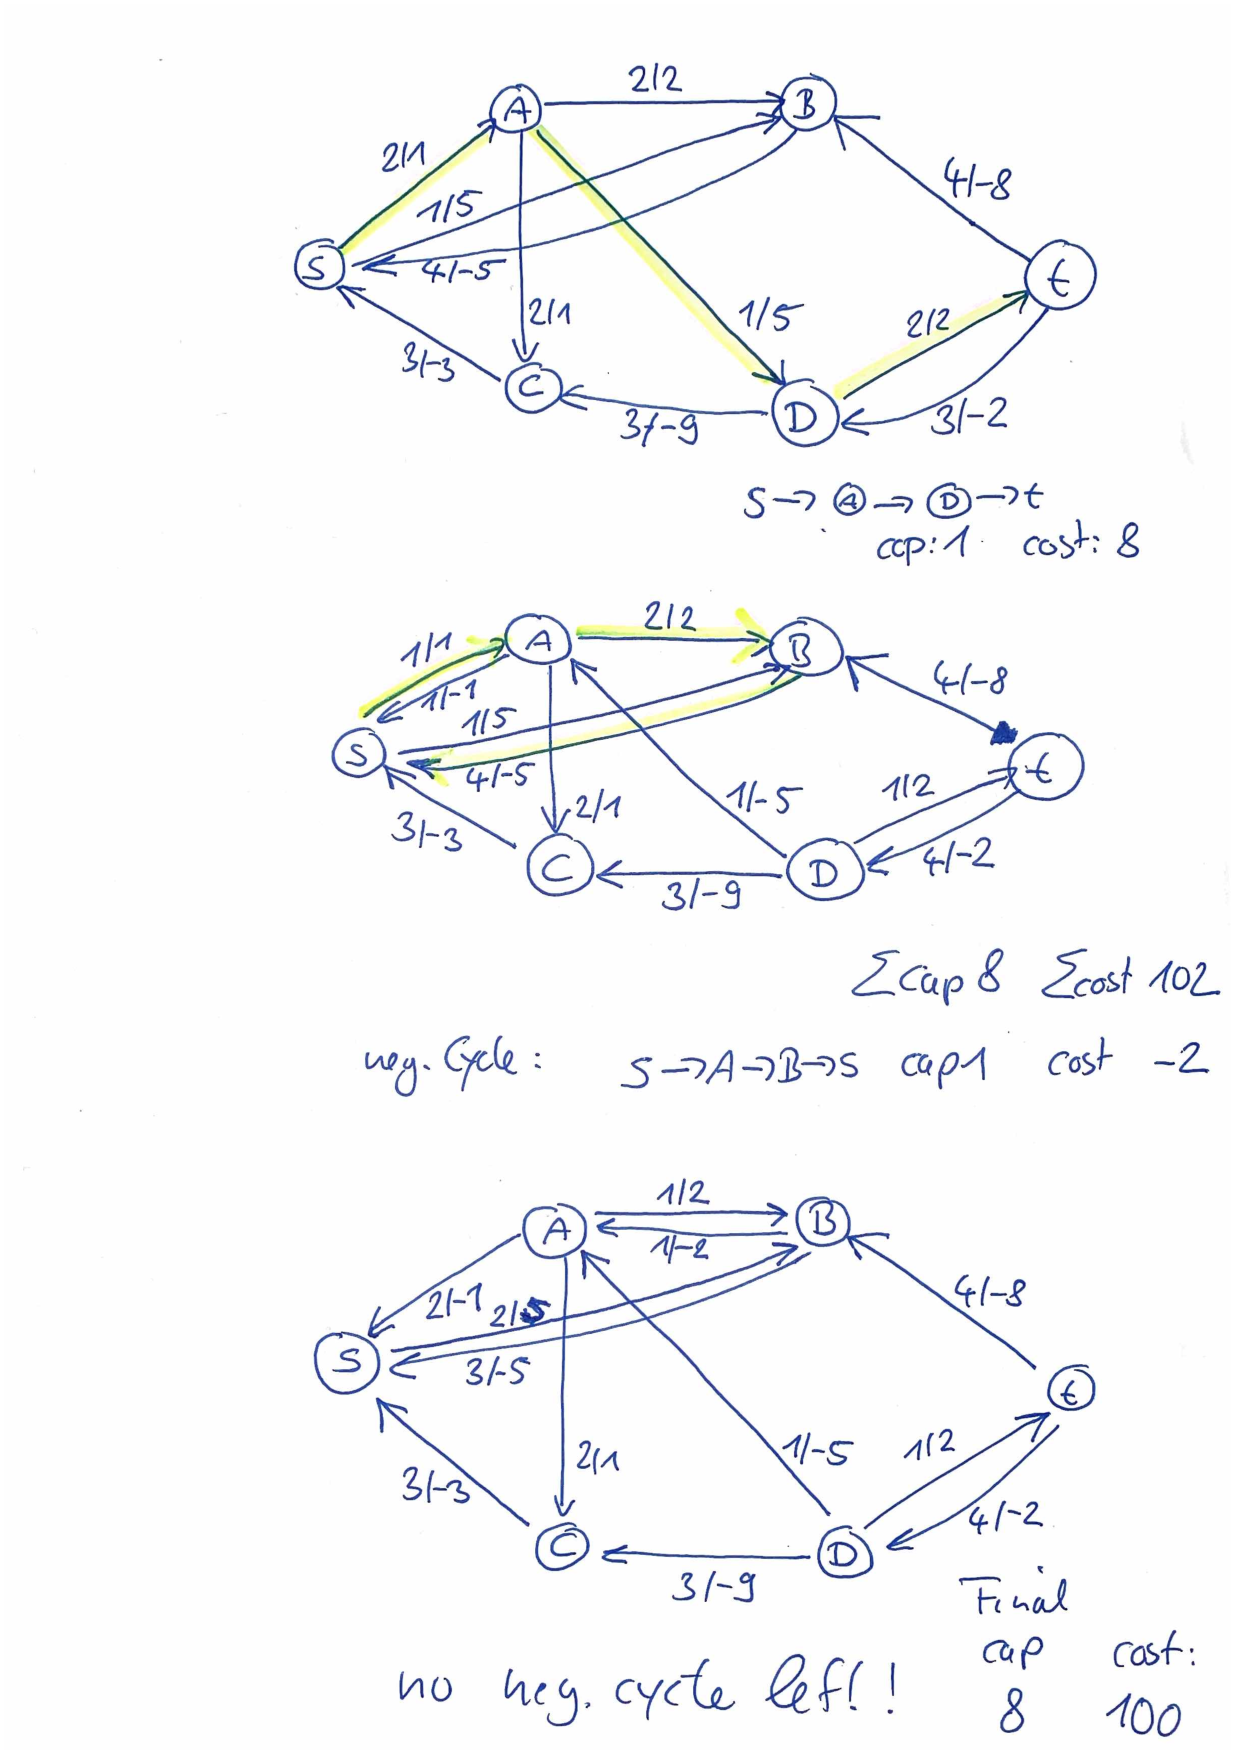
\includepdf[pages=1]{./Content/Examples/example_maxflow2.pdf}
\end{figure}


\newpage
\begin{figure}[h]
	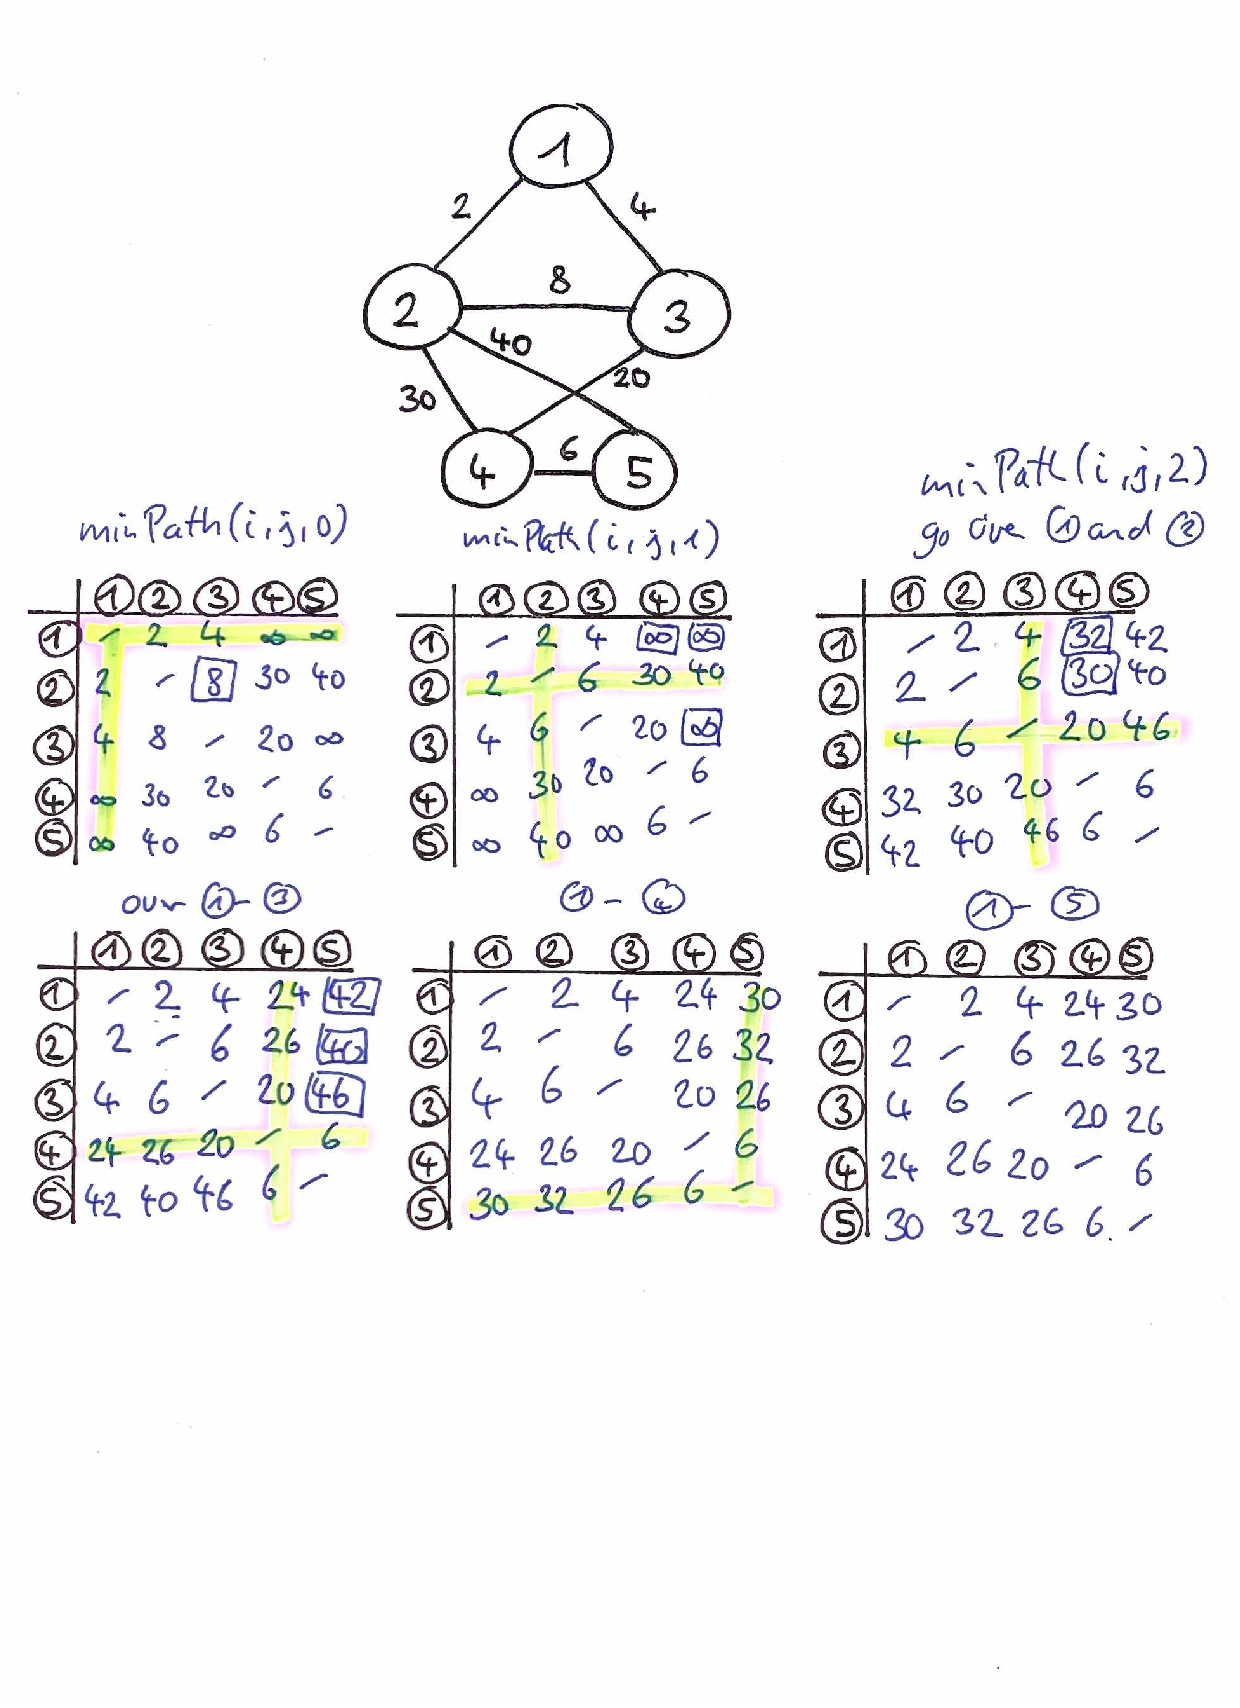
\includepdf[pages=1]{./Content/Examples/example_floydwarshall.pdf}
\end{figure}

